% Provenance (never printed): old premiere S material on subduction (Wadati-Benioff
% planes, density of the old lithosphere, slab pull, transformation of the slab at
% depth: blueschist and eclogite; anatomy of an active margin). Sections from
% figdata/grade-11/slab_sections.py (USGS ComCat M >= 6 1976-2025, PB2002 steps,
% Seton 2020 ages); plate speeds from plate_velocities.py (NNR-MORVEL56 RMS).
% Metamorphism is defined in g12.03, the volcanic arc in g12.04: named only here.
\chapter{Las zonas de subducción}\label{ch:g11:subduction-zones}

Bajo las islas Tonga, en el suroeste del Pacífico, la Tierra tiembla a mucha
más profundidad que en ningún otro lugar. De los siete mil terremotos de
magnitud 6 o más registrados en todo el mundo entre 1976 y 2025, el más
profundo se produjo a \qty{688}{km}, y el corte a través de Tonga de este capítulo contiene sucesos
hasta unos \qty{671}{km}. A esas profundidades la roca está caliente y
sometida a una presión enorme; debería fluir lentamente, como la \omterm{def:g11:lithosphere-asthenosphere:lithosphere}{astenosfera},
y no romperse. Sin embargo, se rompe. Este capítulo explica qué hay allí que
pueda romperse: una \omterm{def:g11:subduction-zones:slab}{losa} de fondo oceánico frío que vuelve a hundirse en el
manto.
% ledger: data:usgs-comcat (catalogue_maxdepth 688; tonga_maxdepth 670.8, slab_sections.py)

\begin{recall}
En un límite convergente, dos placas se mueven una hacia la otra; algunos
están bordeados por fosas profundas (Libro 1, años 7 y 8). La magnitud de un
terremoto mide su tamaño, y un terremoto bajo el mar puede provocar un
tsunami (Libro 1, año 7). La velocidad de una placa respecto de otra es la
diferencia de sus velocidades (el \cref{ch:g11:plate-motions}). El fondo
oceánico se hunde a medida que envejece, y al cabo de unos 60 millones de
años su \omterm{def:g11:lithosphere-asthenosphere:lithosphere}{litosfera}, de unos \qty{100}{km} de espesor, es más densa que la
\omterm{def:g11:lithosphere-asthenosphere:lithosphere}{astenosfera} que tiene debajo (el \cref{ch:g11:ocean-ridges}). Las ondas
sísmicas muestran un cambio brusco en el manto a unos \qty{670}{km} (el
\cref{ch:g11:seismic-structure}). Una roca metamórfica es una roca
transformada en estado sólido (Libro 1, año 6).
\end{recall}
% ledger: data:prem (670 km), ps77:depth-age

\section{Fosas y zonas inclinadas de terremotos}

La mayoría de los terremotos son someros: en el catálogo de magnitud 6 o más
desde 1976, solo alrededor de uno de cada cinco está a más de \qty{70}{km} de
profundidad, y uno de cada quince a más de \qty{300}{km}. El mapa siguiente
muestra dónde están los profundos.
% values (slab_sections.py): frac_deeper_70 0.21, frac_deeper_300 0.069; data:usgs-comcat

\begin{omfigure}
\begin{tikzpicture}
\begin{axis}[ommap, width=\linewidth, xtick={-180,-90,...,180}, ytick={-60,0,60},
  legend style={font=\scriptsize, at={(0.5,-0.13)}, anchor=north, legend columns=3,
    /tikz/every even column/.append style={column sep=6pt}}]
\addplot[fill=omLithAlluv, draw=black!45, line width=0.2pt, forget plot] table {figdata/out/shared-geo-land.dat};
\addplot[black!70, line width=0.5pt, forget plot] table {figdata/out/shared-geo-school-subduction.dat};
\addplot[fill=black!70, draw=none, forget plot] table {figdata/out/shared-geo-school-teeth.dat};
% computed in figdata/grade-11/slab_sections.py; ledger: data:usgs-comcat, data:pb2002
\addplot[only marks, mark=*, mark size=0.55pt, black!45] table[x=lon, y=lat] {figdata/out/grade-11-slab_sections-world-shallow.dat};
\addplot[only marks, mark=*, mark size=0.8pt, omProp] table[x=lon, y=lat] {figdata/out/grade-11-slab_sections-world-mid.dat};
\addplot[only marks, mark=*, mark size=1.1pt, omThm] table[x=lon, y=lat] {figdata/out/grade-11-slab_sections-world-deep.dat};
\legend{{a menos de \qty{70}{km}}, {de 70 a \qty{300}{km}}, {a más de \qty{300}{km}}}
\end{axis}
\end{tikzpicture}

{\small Terremotos de magnitud 6.5 o más, 1976--2025 (2192 sucesos),
coloreados según su profundidad, con las fosas (línea negra, triángulos sobre
la placa cabalgante). Los terremotos intermedios y profundos solo se
encuentran a lo largo de algunas fosas, siempre del lado de la placa
cabalgante. Datos: catálogo de terremotos del USGS; límites de placas de Bird
(2003); tierras emergidas de Natural Earth.}
\end{omfigure}
% values: world_n_m65 2192, world_deep_n 197 (slab_sections.py)

Los terremotos profundos no están dispersos: siguen las fosas del Pacífico
occidental, de Kamchatka a Japón, las Marianas, Indonesia y Tonga, y la fosa
que bordea la costa oeste de América del Sur; y siempre están a un lado de la
fosa, bajo la placa que no se hunde.

\begin{definition}[Subducción; zona de subducción]\label{def:g11:subduction-zones:subduction}
La \emph{subducción}\index{subduccion@subducción} es el hundimiento de una placa de
\omterm{def:g11:ocean-ridges:oceanic-lithosphere}{litosfera oceánica} bajo otra placa, de vuelta al manto. Una \emph{zona de
subducción}\index{zona de subduccion@zona de subducción} es un límite de placas convergente en el
que se produce la subducción; en la superficie la señala una fosa.
\end{definition}

\begin{definition}[Zona de Wadati--Benioff]\label{def:g11:subduction-zones:benioff}
Una \emph{zona de Wadati--Benioff}\index{zona de Wadati--Benioff} es la franja
inclinada de terremotos que empieza en una fosa y se hace cada vez más
profunda bajo la placa cabalgante, hasta unos \qty{700}{km} como mucho.
\end{definition}
% ledger: frohlich87:wadati

\begin{history}[Wadati y Benioff]
En la década de 1920, sismólogos destacados sostenían que los terremotos solo
podían producirse en las primeras decenas de kilómetros: la Tierra más
profunda, razonaban, no tenía resistencia para acumular la deformación. El sismólogo japonés Kiyoo Wadati, que trabajaba con la
densa red de estaciones de la Agencia Meteorológica de Japón, aportó a partir
de 1928 las primeras pruebas convincentes de que algunos terremotos están a
cientos de kilómetros de profundidad: uno de los sucesos que estudió, en
enero de 1927, estaba a \qty{420}{km}. En 1935 publicó el primer mapa de las
profundidades de estos terremotos, trazado con curvas de nivel, y observó que
la zona que se hacía más profunda corría paralela a la línea de volcanes
activos. En 1949 y 1954, el sismólogo estadounidense Hugo Benioff mostró que
bajo los Andes y las islas Tonga--Kermadec los terremotos se sitúan a lo largo
de zonas que alcanzan unos \qty{700}{km} de profundidad. Las zonas se
llamaron primero zonas de Benioff, en 1967; el nombre de \omterm{def:g11:subduction-zones:benioff}{zona de
Wadati--Benioff}, que reconoce el mérito de ambos, sigue una propuesta del
geofísico japonés Seiya Uyeda en 1971.
\end{history}
% ledger: frohlich87:wadati

\begin{method}[Leer un corte de terremotos]\label{met:g11:subduction-zones:section}
\begin{enumerate}
  \item Elige una línea perpendicular a la fosa, desde la fosa hacia la placa
        cabalgante, y conserva los terremotos situados dentro de una franja a
        cada lado de ella.
  \item Representa cada terremoto en su distancia a lo largo de la línea (en
        horizontal) y en su profundidad (en vertical, hacia abajo).
  \item Busca la franja inclinada; traza la recta que mejor la sigue.
  \item Lee el buzamiento de la franja a partir de dos puntos de la recta
        (proposición siguiente).
\end{enumerate}
\end{method}

\begin{omfigure}
\begin{tikzpicture}
\begin{axis}[omrecord, omdepth, name=tonga, width=0.5\linewidth, height=6.4cm,
  xmin=-150, xmax=900, ymin=0, ymax=720, xlabel={distancia a la fosa (\unit{km})},
  ylabel={profundidad (\unit{km})}, title={\small Tonga}, clip=false]
% computed in figdata/grade-11/slab_sections.py; ledger: data:usgs-comcat, data:pb2002
\addplot[only marks, mark=*, mark size=1.2pt, black!65] table[x=x, y=depth] {figdata/out/grade-11-slab_sections-tonga.dat};
\addplot[omProp, line width=1pt, domain=135.7:761.6, samples=2] {-23.568 + 0.91068*x};
\addplot[only marks, mark=triangle*, mark size=3pt, omDef] coordinates {(0,0)};
\node[font=\scriptsize, anchor=south west, text=omDef] at (axis cs:10,8) {fosa};
\node[font=\scriptsize, anchor=east, text=omProp, align=right] at (axis cs:300,560) {buzamiento\\\ang{42}};
\end{axis}
\begin{axis}[omrecord, omdepth, at={(tonga.east)}, anchor=west, xshift=0.3cm, width=0.5\linewidth, height=6.4cm,
  xmin=-150, xmax=900, ymin=0, ymax=720, xlabel={distancia a la fosa (\unit{km})},
  yticklabels={}, title={\small Andes, hacia \ang{21} S}, clip=false]
\addplot[only marks, mark=*, mark size=1.2pt, black!65] table[x=x, y=depth] {figdata/out/grade-11-slab_sections-andes.dat};
\addplot[omProp, line width=1pt, domain=253.0:900, samples=2] {-88.745 + 0.74613*x};
\addplot[only marks, mark=triangle*, mark size=3pt, omDef] coordinates {(0,0)};
\node[font=\scriptsize, anchor=south west, text=omDef] at (axis cs:10,8) {fosa};
\node[font=\scriptsize, anchor=east, text=omProp, align=right] at (axis cs:300,560) {buzamiento\\\ang{37}};
\end{axis}
\end{tikzpicture}

{\small Cortes de terremotos perpendiculares a dos fosas: terremotos de
magnitud 6 o más, 1976--2025, situados a menos de \qty{150}{km} de la línea
del corte, representados en su distancia a la fosa (hacia la placa
cabalgante) y en su profundidad. Naranja: la recta que mejor sigue los
terremotos entre 100 y \qty{600}{km} de profundidad. Bajo Tonga la franja
llega por debajo de \qty{670}{km}. Datos: catálogo de terremotos del USGS; posiciones de las fosas según Bird (2003).}
\end{omfigure}
% values (slab_sections.py): tonga_dip 42.3, fit -23.568 + 0.91068 x (77 events);
% andes_dip 36.7, fit -88.745 + 0.74613 x; trench points tonga (-173.31, -20.395),
% andes (-71.286, -21.01)

\begin{proposition}[El buzamiento de una losa a partir de un corte de terremotos]\label{prop:g11:subduction-zones:dip}
Si dos puntos de la recta que sigue una \omterm{def:g11:subduction-zones:benioff}{zona de Wadati--Benioff} están a
distancias horizontales $x_1 < x_2$ de la fosa y a profundidades $z_1$ y
$z_2$, su buzamiento $\delta$, el ángulo que forma con la horizontal, cumple
\[
  \tan \delta = \frac{z_2 - z_1}{x_2 - x_1}.
\]
\end{proposition}

\begin{proof}
Los dos puntos y el punto situado a la profundidad $z_1$ en la vertical del
segundo forman un triángulo rectángulo. Su cateto horizontal es $x_2 - x_1$,
su cateto vertical $z_2 - z_1$, y el ángulo en el primer punto es el
buzamiento. La tangente de un ángulo de un triángulo rectángulo es el cateto
opuesto dividido entre el cateto contiguo.
\end{proof}

\begin{example}[El buzamiento bajo Tonga]\label{ex:g11:subduction-zones:dip}
La recta del corte de Tonga pasa a \qty{250}{km} de profundidad a
\qty{300}{km} de la fosa y a \qty{614}{km} de profundidad a \qty{700}{km}. Así,
$\tan\delta = (614 - 250)/(700 - 300) = 364/400 = 0.91$, y
$\delta \approx \ang{42}$. Bajo los Andes, a \ang{21}~S, el mismo
método da unos \ang{37}.
\end{example}
% values: tonga line at 300 km 249.6, at 700 km 613.9 (slab_sections.py)

La \omterm{def:g11:subduction-zones:benioff}{zona de Wadati--Benioff} dibuja una placa que desciende. Los terremotos
someros se producen donde las dos placas rozan una contra otra, cerca de la
fosa; los más profundos, dentro de la propia placa que se hunde.

\section{Por qué se hunde la litosfera antigua}

\begin{definition}[Losa]\label{def:g11:subduction-zones:slab}
Una \emph{losa}\index{losa} es la parte de una placa que ya se ha hundido en
el manto en una \omterm{def:g11:subduction-zones:subduction}{zona de subducción}: una lámina de \omterm{def:g11:ocean-ridges:oceanic-lithosphere}{litosfera oceánica}, de unos
cien kilómetros de espesor, inclinada bajo la placa cabalgante.
\end{definition}

Lo que desciende es fondo oceánico antiguo. Según la edad del fondo oceánico,
el fondo que llega a la fosa de Japón, al este de Japón, tiene unos 133
millones de años, y el que llega a la fosa de Tonga, unos 99 millones de
años; incluso el fondo que llega a los Andes, de los más jóvenes que se
hunden, tiene unos 49 millones de años. Una \omterm{def:g11:lithosphere-asthenosphere:lithosphere}{litosfera} tan antigua es fría y
gruesa y, salvo su corteza ligera, más densa que la \omterm{def:g11:lithosphere-asthenosphere:lithosphere}{astenosfera}: en cuanto uno
de sus bordes empieza a descender, su propio peso tira de ella hacia abajo.
% values (slab_sections.py): japan_age 133.1, tonga_age 98.8, andes_age 48.8 (median of the
% 1-degree cells 100-400 km seaward of the trench point); ledger data:b2-seafloor-age

\begin{definition}[Tirón de la losa; empuje de la dorsal]\label{def:g11:subduction-zones:slab-pull}
El \emph{tirón de la losa}\index{tiron de la losa@tirón de la losa} es la fuerza que una \omterm{def:g11:subduction-zones:slab}{losa}
que se hunde, más densa que el manto que la rodea, ejerce sobre el resto de su
placa, y que tira de ella hacia la fosa. El \emph{empuje de la dorsal}\index{empuje de la dorsal} es la fuerza que aleja una
placa de una dorsal, donde la \omterm{def:g11:lithosphere-asthenosphere:lithosphere}{litosfera} joven y caliente está alta sobre su
dorsal elevada y se desliza por su pendiente.
\end{definition}

¿Cuál de las dos importa más? En 1975, Donald Forsyth y Seiya Uyeda
calcularon la intensidad de cada fuerza a partir de las velocidades y las
formas de las placas: las fuerzas sobre las \omterm{def:g11:subduction-zones:slab}{losas} que se hunden controlan la velocidad de las placas oceánicas,
y son unas diez veces más intensas que cualquier otra fuerza. Las velocidades
actuales de las placas lo muestran con claridad.
% ledger: fu75:slab-pull

\begin{omfigure}
\begin{tikzpicture}
\begin{axis}[omrecord, ybar, bar width=9pt, width=0.86\linewidth, height=5.6cm,
  ymin=0, ymax=85, xmin=-0.7, xmax=12.7, bar shift=0pt, ylabel={velocidad media (\unit{mm} al año)},
  xtick={0,...,12}, xticklabel style={rotate=50, anchor=east, font=\scriptsize},
  xticklabels={Cocos, Nazca, Pacífico, Australia, mar de Filipinas, Arabia, Somalia,
    Nubia, Eurasia, América del Norte, Antártida, Caribe, América del Sur},
  ymajorgrids, xmajorgrids=false]
% computed in figdata/grade-11/slab_sections.py from plate_velocities.POLES (nnr56:rms)
\addplot[fill=omProp, draw=omProp!70!black] table[x=idx, y expr=\thisrow{slab}*\thisrow{rms}] {figdata/out/grade-11-slab_sections-speeds.dat};
\addplot[fill=omDef!35, draw=omDef] table[x=idx, y expr=(1-\thisrow{slab})*\thisrow{rms}] {figdata/out/grade-11-slab_sections-speeds.dat};
\node[font=\scriptsize, text=omProp!80!black, anchor=south] at (axis cs:2,76) {una losa cuelga de la placa};
\node[font=\scriptsize, text=omDef, anchor=south] at (axis cs:9,50) {sin losa larga};
\end{axis}
\end{tikzpicture}

{\small Velocidad media de trece grandes placas (media cuadrática sobre la
placa, en un marco en el que la \omterm{def:g11:lithosphere-asthenosphere:lithosphere}{litosfera} en su conjunto no gira). Naranja:
placas de las que cuelga una \omterm{def:g11:subduction-zones:slab}{losa} que se hunde a lo largo de un tramo largo
de su borde; azul: placas sin ella. Se deja fuera la India: su borde norte es
una colisión. Datos: NNR-MORVEL56 (Argus, Gordon y DeMets,
2011).}
\end{omfigure}
% ledger: nnr56:rms; the bars of a class are drawn at 0 for the other (two series on one axis)

\begin{proposition}[Las placas unidas a losas son rápidas]\label{prop:g11:subduction-zones:fast}
Las cinco grandes placas de las que cuelga una \omterm{def:g11:subduction-zones:slab}{losa} larga (Cocos, Nazca,
Pacífico, Australia, mar de Filipinas) se mueven de media a unos
\qty{65}{mm} al año; las ocho que no la tienen, a unos \qty{24}{mm} al año,
casi tres veces más despacio. Cada placa del primer grupo es más rápida que
todas las del segundo.
\end{proposition}
% values: rms_slab_mean 65.2, rms_noslab_mean 23.9 (plate_velocities.py); India left out
% (its northern edge is a collision)

\begin{proof}
A partir de las velocidades medias publicadas, las placas con \omterm{def:g11:subduction-zones:slab}{losa} dan
$(74.6 + 70.0 + 65.5 + 63.1 + 52.6)/5 \approx 65.2$ y las demás
$(47.6 + 31.0 + 29.2 + 22.8 + 19.8 + 15.2 + 14.9 + 10.6)/8 \approx 23.9$
(milímetros al año); la placa con \omterm{def:g11:subduction-zones:slab}{losa} más lenta, la del mar de Filipinas, con
52.6, es más rápida que la más rápida de las demás, Arabia, con 47.6.
\end{proof}
% ledger: nnr56:rms

\section{La losa transformada en profundidad}

Mientras la \omterm{def:g11:subduction-zones:slab}{losa} desciende, su corteza de basalto y \omterm{def:g11:ocean-ridges:gabbro}{gabro} queda enterrada cada
vez más hondo sin dejar de estar fría, porque la \omterm{def:g11:subduction-zones:slab}{losa} se hunde más deprisa de
lo que el calor puede llegar a su interior. Las rocas de la corteza cambian
de minerales sin fundirse: se metamorfizan (el \cref{ch:g12:metamorphic-rocks}).
Dos rocas señalan el camino.

\begin{definition}[Esquisto azul; eclogita]\label{def:g11:subduction-zones:eclogite}
El \emph{esquisto azul}\index{esquisto azul} es una roca metamórfica formada a
partir del basalto de la \omterm{def:g11:ocean-ridges:oceanic-lithosphere}{corteza oceánica} enterrado a alta presión mientras
sigue relativamente frío; lo colorea de azul el mineral glaucofana. La \emph{eclogita}\index{eclogita}
es la roca metamórfica densa en la que se convierten el basalto y el \omterm{def:g11:ocean-ridges:gabbro}{gabro} a
las profundidades del manto a lo largo de las \omterm{def:g11:subduction-zones:subduction}{zonas de subducción}: tiene la
misma composición química, pero está formada por granate rojo y piroxeno verde.
\end{definition}
% ledger: photo:g11-blueschist, photo:g11-eclogite

\begin{omfigure}
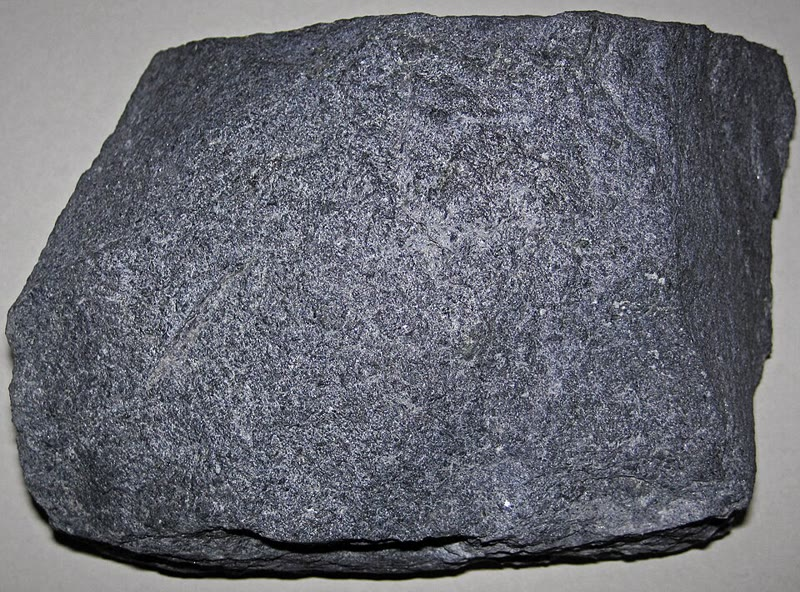
\includegraphics[height=4.4cm]{images/book2/g11-stjohn-blueschist.jpg}\hspace{0.03\linewidth}%
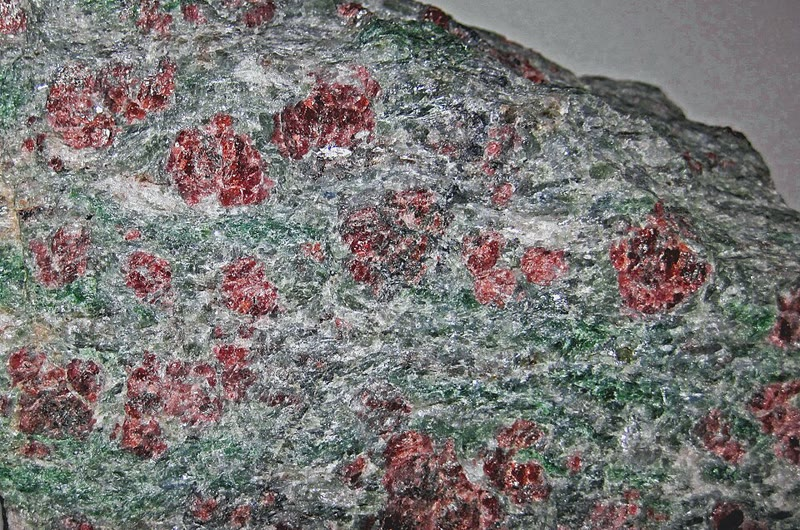
\includegraphics[height=4.4cm]{images/book2/g11-stjohn-eclogite.jpg}

{\small A la izquierda: \omterm{def:g11:subduction-zones:eclogite}{esquisto azul} de la isla Santa Catalina, en California,
antigua \omterm{def:g11:ocean-ridges:oceanic-lithosphere}{corteza oceánica} enterrada en una \omterm{def:g11:subduction-zones:subduction}{zona de subducción}. A la derecha:
\omterm{def:g11:subduction-zones:eclogite}{eclogita} de Noruega, con granates rojos en piroxeno verde. Fotografías de
James St.~John (CC~BY~2.0).}
\end{omfigure}
% ledger: photo:g11-blueschist, photo:g11-eclogite

La \omterm{def:g11:subduction-zones:eclogite}{eclogita} es más densa que el basalto; es incluso más densa que la
\omterm{def:g11:ocean-ridges:peridotite}{peridotita} del manto, en alrededor de un \qty{6}{\percent}. Cuando su corteza
se ha convertido en \omterm{def:g11:subduction-zones:eclogite}{eclogita}, la \omterm{def:g11:subduction-zones:slab}{losa} ya no lleva encima una capa ligera: toda
la \omterm{def:g11:subduction-zones:slab}{losa} es más densa que el manto que la rodea, y tira con más fuerza. Las
rocas de este tipo, devueltas a la superficie por movimientos posteriores, son
de los pocos testigos directos de lo que ocurre a decenas de kilómetros de
profundidad en una \omterm{def:g11:subduction-zones:subduction}{zona de subducción}.
% ledger: hacker03:eclogite, photo:g11-eclogite

\begin{omfigure}
\begin{tikzpicture}[font=\footnotesize, scale=0.85]
  % subduction zone, a drawing, not to scale: slab top flat to x = -1, then bends to a 42-degree dip
  % coordinates computed once by a small script (scratch, not kept): slab top flat to x=-1, arc R=3 to a 42-degree dip
  \fill[omProp!10] (-7,-1.4) rectangle (7,-6.0);
  \fill[omSea!45] (-7,0) -- (-1,0) -- (1.6,0.8) -- (-7,0.8) -- cycle;
  \fill[lith peridotite] (-7.000,0.000) -- (-6.644,0.000) -- (-6.289,0.000) -- (-5.933,0.000) -- (-5.578,0.000) -- (-5.222,0.000) -- (-4.867,0.000) -- (-4.511,0.000) -- (-4.156,0.000) -- (-3.800,0.000) -- (-3.445,0.000) -- (-3.089,0.000) -- (-2.734,0.000) -- (-2.378,0.000) -- (-2.023,0.000) -- (-1.667,0.000) -- (-1.312,0.000) -- (-0.956,-0.000) -- (-0.602,-0.027) -- (-0.253,-0.094) -- (0.085,-0.203) -- (0.408,-0.351) -- (0.712,-0.536) -- (0.991,-0.756) -- (1.255,-0.994) -- (1.519,-1.232) -- (1.784,-1.470) -- (2.048,-1.707) -- (2.312,-1.945) -- (2.576,-2.183) -- (2.840,-2.421) -- (3.105,-2.659) -- (3.369,-2.897) -- (3.633,-3.135) -- (3.897,-3.373) -- (4.161,-3.611) -- (4.426,-3.848) -- (4.690,-4.086) -- (4.954,-4.324) -- (5.218,-4.562) -- (5.483,-4.800) -- (4.546,-5.840) -- (4.282,-5.603) -- (4.017,-5.365) -- (3.753,-5.127) -- (3.489,-4.889) -- (3.225,-4.651) -- (2.961,-4.413) -- (2.696,-4.175) -- (2.432,-3.937) -- (2.168,-3.699) -- (1.904,-3.461) -- (1.639,-3.224) -- (1.375,-2.986) -- (1.111,-2.748) -- (0.847,-2.510) -- (0.583,-2.272) -- (0.318,-2.034) -- (0.062,-1.803) -- (-0.087,-1.686) -- (-0.249,-1.587) -- (-0.421,-1.508) -- (-0.602,-1.450) -- (-0.788,-1.414) -- (-0.977,-1.400) -- (-1.312,-1.400) -- (-1.667,-1.400) -- (-2.023,-1.400) -- (-2.378,-1.400) -- (-2.734,-1.400) -- (-3.089,-1.400) -- (-3.445,-1.400) -- (-3.800,-1.400) -- (-4.156,-1.400) -- (-4.511,-1.400) -- (-4.867,-1.400) -- (-5.222,-1.400) -- (-5.578,-1.400) -- (-5.933,-1.400) -- (-6.289,-1.400) -- (-6.644,-1.400) -- (-7.000,-1.400) -- cycle;
  \fill[lith basalt] (-7.000,0.000) -- (-6.644,0.000) -- (-6.289,0.000) -- (-5.933,0.000) -- (-5.578,0.000) -- (-5.222,0.000) -- (-4.867,0.000) -- (-4.511,0.000) -- (-4.156,0.000) -- (-3.800,0.000) -- (-3.445,0.000) -- (-3.089,0.000) -- (-2.734,0.000) -- (-2.378,0.000) -- (-2.023,0.000) -- (-1.667,0.000) -- (-1.312,0.000) -- (-0.956,-0.000) -- (-0.602,-0.027) -- (-0.253,-0.094) -- (0.085,-0.203) -- (0.408,-0.351) -- (0.712,-0.536) -- (0.991,-0.756) -- (1.255,-0.994) -- (1.519,-1.232) -- (1.784,-1.470) -- (2.048,-1.707) -- (2.312,-1.945) -- (2.576,-2.183) -- (2.840,-2.421) -- (3.105,-2.659) -- (3.369,-2.897) -- (3.633,-3.135) -- (3.897,-3.373) -- (4.161,-3.611) -- (4.426,-3.848) -- (4.690,-4.086) -- (4.954,-4.324) -- (5.218,-4.562) -- (5.483,-4.800) -- (5.282,-5.023) -- (5.018,-4.785) -- (4.753,-4.547) -- (4.489,-4.309) -- (4.225,-4.071) -- (3.961,-3.833) -- (3.697,-3.596) -- (3.432,-3.358) -- (3.168,-3.120) -- (2.904,-2.882) -- (2.640,-2.644) -- (2.376,-2.406) -- (2.111,-2.168) -- (1.847,-1.930) -- (1.583,-1.692) -- (1.319,-1.455) -- (1.054,-1.217) -- (0.792,-0.980) -- (0.541,-0.783) -- (0.268,-0.616) -- (-0.023,-0.483) -- (-0.328,-0.385) -- (-0.642,-0.324) -- (-0.960,-0.300) -- (-1.312,-0.300) -- (-1.667,-0.300) -- (-2.023,-0.300) -- (-2.378,-0.300) -- (-2.734,-0.300) -- (-3.089,-0.300) -- (-3.445,-0.300) -- (-3.800,-0.300) -- (-4.156,-0.300) -- (-4.511,-0.300) -- (-4.867,-0.300) -- (-5.222,-0.300) -- (-5.578,-0.300) -- (-5.933,-0.300) -- (-6.289,-0.300) -- (-6.644,-0.300) -- (-7.000,-0.300) -- cycle;
  \fill[blue!30] (2.484,-2.100) -- (2.604,-2.208) -- (2.725,-2.317) -- (2.845,-2.425) -- (2.965,-2.533) -- (3.085,-2.642) -- (3.206,-2.750) -- (3.326,-2.858) -- (3.446,-2.967) -- (3.567,-3.075) -- (3.687,-3.183) -- (3.807,-3.292) -- (3.928,-3.400) -- (3.727,-3.623) -- (3.607,-3.515) -- (3.486,-3.406) -- (3.366,-3.298) -- (3.246,-3.190) -- (3.125,-3.081) -- (3.005,-2.973) -- (2.885,-2.865) -- (2.764,-2.756) -- (2.644,-2.648) -- (2.524,-2.540) -- (2.403,-2.431) -- (2.283,-2.323) -- cycle;
  \fill[lith eclogite] (3.928,-3.400) -- (4.057,-3.517) -- (4.187,-3.633) -- (4.316,-3.750) -- (4.446,-3.867) -- (4.576,-3.983) -- (4.705,-4.100) -- (4.835,-4.217) -- (4.964,-4.333) -- (5.094,-4.450) -- (5.223,-4.567) -- (5.353,-4.683) -- (5.483,-4.800) -- (5.282,-5.023) -- (5.152,-4.906) -- (5.023,-4.790) -- (4.893,-4.673) -- (4.764,-4.556) -- (4.634,-4.440) -- (4.504,-4.323) -- (4.375,-4.206) -- (4.245,-4.090) -- (4.116,-3.973) -- (3.986,-3.856) -- (3.857,-3.740) -- (3.727,-3.623) -- cycle;
  \draw[black!60] (-7.000,0.000) -- (-6.644,0.000) -- (-6.289,0.000) -- (-5.933,0.000) -- (-5.578,0.000) -- (-5.222,0.000) -- (-4.867,0.000) -- (-4.511,0.000) -- (-4.156,0.000) -- (-3.800,0.000) -- (-3.445,0.000) -- (-3.089,0.000) -- (-2.734,0.000) -- (-2.378,0.000) -- (-2.023,0.000) -- (-1.667,0.000) -- (-1.312,0.000) -- (-0.956,-0.000) -- (-0.602,-0.027) -- (-0.253,-0.094) -- (0.085,-0.203) -- (0.408,-0.351) -- (0.712,-0.536) -- (0.991,-0.756) -- (1.255,-0.994) -- (1.519,-1.232) -- (1.784,-1.470) -- (2.048,-1.707) -- (2.312,-1.945) -- (2.576,-2.183) -- (2.840,-2.421) -- (3.105,-2.659) -- (3.369,-2.897) -- (3.633,-3.135) -- (3.897,-3.373) -- (4.161,-3.611) -- (4.426,-3.848) -- (4.690,-4.086) -- (4.954,-4.324) -- (5.218,-4.562) -- (5.483,-4.800);
  \draw[black!60] (-7.000,-1.400) -- (-6.644,-1.400) -- (-6.289,-1.400) -- (-5.933,-1.400) -- (-5.578,-1.400) -- (-5.222,-1.400) -- (-4.867,-1.400) -- (-4.511,-1.400) -- (-4.156,-1.400) -- (-3.800,-1.400) -- (-3.445,-1.400) -- (-3.089,-1.400) -- (-2.734,-1.400) -- (-2.378,-1.400) -- (-2.023,-1.400) -- (-1.667,-1.400) -- (-1.312,-1.400) -- (-0.977,-1.400) -- (-0.788,-1.414) -- (-0.602,-1.450) -- (-0.421,-1.508) -- (-0.249,-1.587) -- (-0.087,-1.686) -- (0.062,-1.803) -- (0.318,-2.034) -- (0.583,-2.272) -- (0.847,-2.510) -- (1.111,-2.748) -- (1.375,-2.986) -- (1.639,-3.224) -- (1.904,-3.461) -- (2.168,-3.699) -- (2.432,-3.937) -- (2.696,-4.175) -- (2.961,-4.413) -- (3.225,-4.651) -- (3.489,-4.889) -- (3.753,-5.127) -- (4.017,-5.365) -- (4.282,-5.603) -- (4.546,-5.840);
  \draw[black!60] (5.483,-4.800) -- (4.546,-5.840);
  \fill[omLithGranite!55] (-1.000,0.000) -- (1.600,0.800) -- (7.000,0.800) -- (7.000,-1.600) -- (1.929,-1.600) -- (1.801,-1.485) -- (1.673,-1.370) -- (1.545,-1.255) -- (1.417,-1.140) -- (1.290,-1.025) -- (1.162,-0.910) -- (1.034,-0.795) -- (0.904,-0.682) -- (0.768,-0.577) -- (0.627,-0.479) -- (0.480,-0.390) -- (0.328,-0.310) -- (0.172,-0.238) -- (0.011,-0.176) -- (-0.152,-0.122) -- (-0.318,-0.078) -- (-0.487,-0.044) -- (-0.657,-0.020) -- (-0.828,-0.005) -- (-1.000,0.000) -- cycle;
  \fill[omLithAlluv] (-1.000,0.000) -- (0.550,0.470) -- (0.926,-0.700) -- (0.761,-0.571) -- (0.588,-0.455) -- (0.407,-0.350) -- (0.219,-0.259) -- (0.025,-0.180) -- (-0.174,-0.116) -- (-0.377,-0.065) -- (-0.583,-0.029) -- (-0.791,-0.007) -- (-1.000,0.000) -- cycle;
  \draw[black!60] (-1.000,0.000) -- (1.600,0.800) -- (7.000,0.800) -- (7.000,-1.600) -- (1.929,-1.600) -- (1.801,-1.485) -- (1.673,-1.370) -- (1.545,-1.255) -- (1.417,-1.140) -- (1.290,-1.025) -- (1.162,-0.910) -- (1.034,-0.795) -- (0.904,-0.682) -- (0.768,-0.577) -- (0.627,-0.479) -- (0.480,-0.390) -- (0.328,-0.310) -- (0.172,-0.238) -- (0.011,-0.176) -- (-0.152,-0.122) -- (-0.318,-0.078) -- (-0.487,-0.044) -- (-0.657,-0.020) -- (-0.828,-0.005) -- (-1.000,0.000);
  \draw[omThm!75, densely dashed, line width=0.7pt] (-7.000,-1.150) -- (-6.648,-1.150) -- (-6.296,-1.150) -- (-5.945,-1.150) -- (-5.593,-1.150) -- (-5.241,-1.150) -- (-4.889,-1.150) -- (-4.538,-1.150) -- (-4.186,-1.150) -- (-3.834,-1.150) -- (-3.482,-1.150) -- (-3.130,-1.150) -- (-2.779,-1.150) -- (-2.427,-1.150) -- (-2.075,-1.150) -- (-1.723,-1.150) -- (-1.372,-1.150) -- (-1.020,-1.150) -- (-0.796,-1.161) -- (-0.582,-1.198) -- (-0.374,-1.259) -- (-0.175,-1.344) -- (0.013,-1.452) -- (0.187,-1.581) -- (0.419,-1.788) -- (0.680,-2.023) -- (0.942,-2.259) -- (1.203,-2.494) -- (1.465,-2.730) -- (1.726,-2.965) -- (1.987,-3.200) -- (2.249,-3.436) -- (2.510,-3.671) -- (2.772,-3.907) -- (3.033,-4.142) -- (3.294,-4.377) -- (3.556,-4.613) -- (3.817,-4.848) -- (4.079,-5.083) -- (4.340,-5.319) -- (4.602,-5.554) -- (5.103,-4.997) -- (5.045,-4.944) -- (4.987,-4.892) -- (4.929,-4.839) -- (4.870,-4.787) -- (4.812,-4.734) -- (4.754,-4.682) -- (4.695,-4.629) -- (4.637,-4.577) -- (4.579,-4.524) -- (4.520,-4.472) -- (4.462,-4.419) -- (4.404,-4.367) -- (4.346,-4.315) -- (4.287,-4.262) -- (4.229,-4.210) -- (4.171,-4.157) -- (4.112,-4.105) -- (4.054,-4.052) -- (3.996,-4.000) -- (3.937,-3.947) -- (3.879,-3.895) -- (3.821,-3.842) -- (3.763,-3.790) -- (3.704,-3.737) -- (3.646,-3.685) -- (3.588,-3.632) -- (3.529,-3.580) -- (3.471,-3.527) -- (3.413,-3.475) -- (3.355,-3.422) -- (3.296,-3.370) -- (3.238,-3.317) -- (3.180,-3.265) -- (3.121,-3.212) -- (3.063,-3.160) -- (3.005,-3.107) -- (2.946,-3.055) -- (2.888,-3.002) -- (2.830,-2.950) -- (2.772,-2.897) -- (7.000,-2.897);
  \foreach \p in {(-0.72,-0.22),(-0.46,-0.36),(-0.18,-0.37),(0.05,-0.55),(0.29,-0.67),(0.63,-0.66),(0.87,-0.82),(0.91,-1.23),(1.27,-1.29),(1.50,-1.49),(1.55,-1.89),(1.90,-1.96),(2.04,-2.25),(2.35,-2.36),(2.54,-2.61),(2.88,-2.69),(2.99,-3.02),(3.16,-3.28),(3.47,-3.40),(3.65,-3.66),(3.89,-3.84),(4.26,-3.89),(4.32,-4.27),(4.59,-4.43),(4.88,-4.56),(5.17,-4.70)} \fill[black] \p circle (1.3pt);
  % volcanic arc above the slab, back-arc stretched
  \fill[black!70] (3.35,0.8) -- (3.7,1.4) -- (4.05,0.8) -- cycle;
  \draw[black!45, dashed] (5.2,0.8) -- (5.2,-1.6); \draw[black!45, dashed] (6.6,0.8) -- (6.6,-1.6);
  \draw[{Stealth[length=4pt]}-{Stealth[length=4pt]}, black!70] (5.35,-0.7) -- (6.45,-0.7);
  % motion arrows
  \draw[-{Stealth[length=5pt]}, line width=1pt] (-5.6,0.4) -- (-3.6,0.4);
  \draw[-{Stealth[length=5pt]}, line width=1pt] (1.77,-4.01) -- (2.88,-5.01);
  % labels
  \draw[black!60] (-1.0,0.02) -- (-1.8,1.05);
  \node[anchor=south] at (-1.8,1.05) {fosa};
  \draw[black!60] (0.1,0.12) -- (0.5,1.05);
  \node[anchor=south, align=center] at (0.6,1.05) {sedimentos\\arrancados};
  \node[anchor=south] at (2.35,0.85) {antearco};
  \node[anchor=south] at (3.7,1.4) {arco volcánico};
  \node[anchor=south] at (5.9,0.85) {trasarco};
  \node[anchor=south] at (-5.4,0.82) {fondo oceánico que va hacia la fosa};
  \draw[black!60] (-7.0,-0.15) -- (-7.25,-0.15);
  \node[anchor=east] at (-7.25,-0.15) {corteza oceánica};
  \draw[black!60] (-7.0,-0.85) -- (-7.25,-0.85);
  \node[anchor=east, align=right] at (-7.25,-0.85) {parte mantélica\\de la litosfera};
  \node at (-3.5,-3.6) {astenosfera};
  \node[rotate=-42] at (3.98,-4.46) {losa};
  \draw[black!60] (3.35,-2.65) -- (4.3,-2.35);
  \node[anchor=west] at (4.3,-2.35) {esquisto azul};
  \draw[black!60] (5.1,-4.3) -- (5.75,-4.6);
  \node[anchor=west] at (5.75,-4.6) {eclogita};
  \node[anchor=north east, text=omThm!80!black, align=right] at (7,-2.95) {línea de igual\\temperatura};
  \fill[black] (-6.8,-5.55) circle (1.3pt);
  \node[anchor=west] at (-6.65,-5.55) {terremotos};
\end{tikzpicture}

{\small Una \omterm{def:g11:subduction-zones:subduction}{zona de subducción} (un dibujo, no a escala). La \omterm{def:g11:ocean-ridges:oceanic-lithosphere}{litosfera oceánica}
antigua se dobla hacia abajo en la fosa y se hunde bajo la placa cabalgante.
Los sedimentos arrancados de su superficie se acumulan contra el borde de la
placa cabalgante; los terremotos siguen la \omterm{def:g11:subduction-zones:slab}{losa} que se hunde; su corteza se
convierte en \omterm{def:g11:subduction-zones:eclogite}{esquisto azul} y luego en \omterm{def:g11:subduction-zones:eclogite}{eclogita}. La \omterm{def:g11:subduction-zones:slab}{losa} sigue más fría que el
manto que la rodea: las líneas de igual temperatura se ven arrastradas hacia
abajo a lo largo de ella. Una línea de volcanes, el arco volcánico, se alza
sobre la \omterm{def:g11:subduction-zones:slab}{losa}.}
\end{omfigure}
% volcanic arc above the slab: told only, defined and sourced in g12.04

\section{La anatomía de una zona de subducción}

Del océano al continente, o al océano siguiente, una \omterm{def:g11:subduction-zones:subduction}{zona de subducción} tiene
siempre las mismas partes.

\begin{itemize}
  \item La \emph{fosa}, donde la placa que se hunde se dobla hacia abajo: los
        lugares más profundos de los océanos.
  \item El \emph{antearco}, entre la fosa y la línea de volcanes. Su borde es
        un montón de sedimentos arrancados de la placa que se hunde; debajo,
        las dos placas se deslizan una contra otra a lo largo del límite de
        placas, una falla de poca inclinación en la que se producen grandes
        terremotos, como el de 2011 frente a Japón (ejemplo siguiente).
  \item El \emph{arco volcánico}, una línea de volcanes paralela a la fosa,
        en islas (Tonga, las Marianas, Japón) o en un continente (los Andes);
        por qué se forma es el tema del \cref{ch:g12:subduction-magmatism}.
  \item Detrás de algunos arcos, un \emph{trasarco}, donde la placa
        cabalgante se estira; detrás de Tonga se está separando.
\end{itemize}
% ledger: bevis95:tonga (back-arc extension at Tonga); usgs:tohoku (largest earthquakes on the
% plate boundary: example below)

Detrás de Tonga, el estiramiento del trasarco lleva el propio arco hacia la
placa del Pacífico, como ha mostrado el posicionamiento por satélite. La velocidad a la que convergen los dos lados de la fosa de Tonga
es, por tanto, mayor que la velocidad propia de cada placa: según el modelo
PB2002, unos \qty{17}{cm} al año hacia \ang{20}~S.
% values: tonga_rate 168.0 (mean of the PB2002 TO/PA steps within 100 km of the profile);
% PB2002 steps along Tonga: 104 to 237 mm/yr; ledger data:pb2002, bevis95:tonga

\begin{example}[El terremoto de Tōhoku, 2011]\label{ex:g11:subduction-zones:tohoku}
El 11~de marzo de 2011, un terremoto de magnitud 9.1 sacudió el mar frente a
la costa nordeste de Honshu, en Japón. Se produjo a unos \qty{25}{km} de
profundidad, en el propio límite de placas, donde la placa del Pacífico, que
se mueve hacia el oeste a unos \qty{83}{mm} al año respecto de la placa que
lleva el norte de Japón, se hunde bajo ella en la fosa de Japón. Los dos lados
de la falla se desplazaron uno respecto del otro hasta 50 a \qty{60}{m}, en
una superficie de unos \qty{400}{km} de largo y \qty{150}{km} de ancho. El
fondo marino de encima se movió con ellos y provocó un tsunami que alcanzó
\qty{38}{m} de altura en la costa; murieron al menos \num{15703} personas y
\num{4647} quedaron desaparecidas. La misma costa había sufrido tsunamis de
esta \omterm{def:g11:subduction-zones:subduction}{zona de subducción} en 1611, 1896 y 1933, y quizá uno tan grande como el
de 2011 en el año 869.
\end{example}
% ledger: usgs:tohoku

\begin{omfigure}
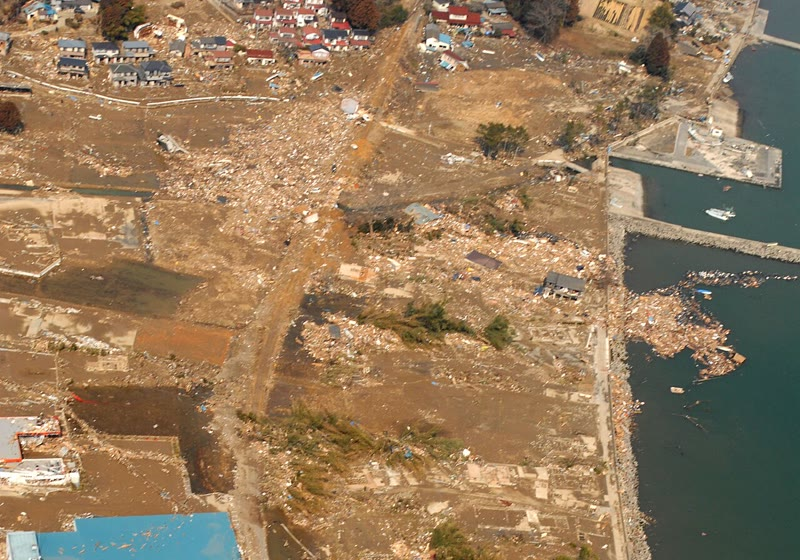
\includegraphics[width=0.78\linewidth]{images/book2/g11-usn-tsunami-kesennuma.jpg}

{\small El puerto pesquero de Kesennuma, en la costa nordeste de Japón, dos
días después del tsunami del 11~de marzo de 2011. Fotografía de Dylan McCord,
U.S. Navy (dominio público).}
\end{omfigure}
% ledger: photo:g11-tsunami

\section{Ejercicios}

\begin{exercise}[$\star$]\label{exo:g11:subduction-zones:1}
Define la \omterm{def:g11:subduction-zones:subduction}{subducción} y una \omterm{def:g11:subduction-zones:subduction}{zona de subducción}. ¿Qué tipo de \omterm{def:g11:lithosphere-asthenosphere:lithosphere}{litosfera} se
hunde en una \omterm{def:g11:subduction-zones:subduction}{zona de subducción}, y por qué ese tipo?
\end{exercise}

\begin{exercise}[$\star$]\label{exo:g11:subduction-zones:2}
Con el mapa mundial de terremotos según su profundidad: (1) nombra tres
regiones con terremotos a más de \qty{300}{km} de profundidad; (2) ¿a qué lado
de una fosa están los terremotos profundos? (3) A lo largo de la dorsal
mesoatlántica, ¿a qué profundidad están los terremotos?
\end{exercise}

\begin{exercise}[$\star$]\label{exo:g11:subduction-zones:3}
El catálogo contiene \num{7031} terremotos de magnitud 6 o más, de los que el
\qty{21}{\percent} están a más de \qty{70}{km} de profundidad y el
\qty{6.9}{\percent} a más de \qty{300}{km}. ¿Cuántos terremotos son en cada caso?
\end{exercise}

\begin{exercise}[$\star$]\label{exo:g11:subduction-zones:4}
Define el \omterm{def:g11:subduction-zones:eclogite}{esquisto azul} y la \omterm{def:g11:subduction-zones:eclogite}{eclogita}. ¿Qué tienen en común los dos con el
basalto de la \omterm{def:g11:ocean-ridges:oceanic-lithosphere}{corteza oceánica}? ¿En qué se diferencian?
\end{exercise}

\begin{exercise}[$\star$]\label{exo:g11:subduction-zones:5}
Enumera en orden las partes de una \omterm{def:g11:subduction-zones:subduction}{zona de subducción}, desde el fondo oceánico
que se mueve hacia la fosa hasta el trasarco, diciendo en una línea qué ocurre
en cada una.
\end{exercise}

\begin{exercise}[$\star\star$]\label{exo:g11:subduction-zones:6}
En el corte de los Andes, la recta que sigue los terremotos pasa a
\qty{135}{km} de profundidad a \qty{300}{km} de la fosa y a \qty{508}{km} de
profundidad a \qty{800}{km}. Calcula el buzamiento de la \omterm{def:g11:subduction-zones:slab}{losa}.
\end{exercise}

\begin{exercise}[$\star\star$]\label{exo:g11:subduction-zones:7}
Una \omterm{def:g11:subduction-zones:slab}{losa} recta empieza en una fosa y buza \ang{45}. (1) ¿A qué profundidad
está a \qty{300}{km} de la fosa? (2) ¿A qué distancia de la fosa llega a
\qty{670}{km}? (3) ¿Qué longitud de \omterm{def:g11:subduction-zones:slab}{losa} hay entre la fosa y
\qty{670}{km}?
\end{exercise}

\begin{exercise}[$\star\star$]\label{exo:g11:subduction-zones:8}
Las velocidades medias de las placas son, en milímetros al año: Cocos 74.6,
Nazca 70.0, Pacífico 65.5, Australia 63.1, mar de Filipinas 52.6 (con \omterm{def:g11:subduction-zones:slab}{losas});
Arabia 47.6, Somalia 31.0, Nubia 29.2, Eurasia 22.8, América del Norte 19.8,
Antártida 15.2, Caribe 14.9, América del Sur 10.6 (sin ellas). (1) Calcula la
media de cada grupo y su cociente. (2) ¿Qué sugiere esto sobre la fuerza que
mueve las placas?
\end{exercise}

\begin{exercise}[$\star\star$]\label{exo:g11:subduction-zones:9}
En 2011, la falla frente a Japón se desplazó hasta 50 a \qty{60}{m}. La placa
del Pacífico se acerca a \qty{83}{mm} al año. (1) ¿Cuántos años de movimiento
de la placa representa un desplazamiento de \qty{50}{m}, y luego uno de
\qty{60}{m}? (2) Compáralo con el tiempo transcurrido desde 869, fecha de un
posible terremoto anterior del mismo tamaño.
\end{exercise}

\begin{exercise}[$\star\star$]\label{exo:g11:subduction-zones:10}
El fondo oceánico que llega a la fosa de Japón tiene unos 133 millones de
años, el que llega a Tonga unos 99 y el que llega a los Andes unos 49. (1) Con
las leyes del \cref{ch:g11:ocean-ridges} ($2500 + 350\sqrt{t}$ para
$t \le 70$, $6400 - 3200\,e^{-t/62.8}$ más allá), halla la profundidad de cada
uno. (2) ¿Cuál es la \omterm{def:g11:lithosphere-asthenosphere:lithosphere}{litosfera} más fría y más densa?
\end{exercise}

\begin{exercise}[$\star\star$]\label{exo:g11:subduction-zones:11}
El basalto de la \omterm{def:g11:ocean-ridges:oceanic-lithosphere}{corteza oceánica} tiene una densidad de unos
\qty{2900}{kg/m^3}, el manto que rodea la \omterm{def:g11:subduction-zones:slab}{losa} \qty{3380}{kg/m^3}, y la
\omterm{def:g11:subduction-zones:eclogite}{eclogita} es un \qty{6}{\percent} más densa que el manto. (1) Halla la densidad
de la \omterm{def:g11:subduction-zones:eclogite}{eclogita}. (2) ¿En qué porcentaje aumenta la densidad de la corteza
cuando se convierte en \omterm{def:g11:subduction-zones:eclogite}{eclogita}? (3) Antes y después, ¿es la corteza más
ligera o más densa que el manto, y en cuánto?
\end{exercise}

\begin{exercise}[$\star\star\star$]\label{exo:g11:subduction-zones:12}
El calor se propaga por conducción a una distancia de unos $\sqrt{\kappa t}$
en un tiempo $t$, con $\kappa = \qty{1e-6}{m^2/s}$ para la roca. (1) Calcula
esta distancia para 6 millones de años ($1~\text{año} \approx \qty{3.16e7}{s}$).
(2) Compárala con el espesor de una \omterm{def:g11:subduction-zones:slab}{losa}, unos \qty{100}{km}. (3) Explica por
qué puede haber terremotos dentro de una \omterm{def:g11:subduction-zones:slab}{losa} a \qty{600}{km} mientras el
manto que la rodea fluye.
\end{exercise}
% ledger: england:kelvin (kappa 1e-6 m2/s)

\begin{exercise}[$\star\star\star$]\label{exo:g11:subduction-zones:13}
Bajo los Andes, a \ang{21}~S, la recta del corte llega a \qty{670}{km} a
\qty{1017}{km} de la fosa, y las placas convergen a \qty{64}{mm} al año.
(1) Estima la longitud de la \omterm{def:g11:subduction-zones:slab}{losa} desde la fosa hasta \qty{670}{km}.
(2) ¿Cuánto tarda un trozo de fondo oceánico en llegar a \qty{670}{km}?
(3) Compáralo con Tonga, donde el mismo viaje dura unos 6 millones de años.
\end{exercise}

\begin{exercise}[$\star\star\star$]\label{exo:g11:subduction-zones:14}
Toma una \omterm{def:g11:subduction-zones:slab}{losa} de \qty{100}{km} de espesor, más densa que el manto que la rodea
en \qty{36}{kg/m^3} de media, y de \qty{1000}{km} de longitud, bajo una fosa.
(1) Calcula el exceso de masa de la \omterm{def:g11:subduction-zones:slab}{losa} por cada metro de fosa. (2) Calcula
su peso, con $g = \qty{9.8}{m/s^2}$. (3) ¿Por qué puede esta fuerza tirar de
toda la placa?
\end{exercise}

\begin{exercise}[$\star\star\star$]\label{exo:g11:subduction-zones:15}
A lo largo de la fosa de Tonga, el modelo PB2002 da una convergencia de
\qty{104}{mm} al año a \ang{23.6}~S y de \qty{237}{mm} al año a
\ang{16.5}~S. (1) ¿Qué distancia separa los dos puntos, a lo largo de un
meridiano ($\ang{1} \approx \qty{111}{km}$)? (2) ¿Cuánto aumenta la velocidad
por cada cien kilómetros? (3) La placa del Pacífico se mueve más o menos a la
misma velocidad en los dos puntos. ¿Qué debe estar haciendo el otro lado de la
fosa, el arco de Tonga?
\end{exercise}

\section{Problema: la losa de Tonga}

\begin{problem}[{Problema de fin de semana --- de la fosa a \qty{670}{km}}]
\label{pb:g11:subduction-zones:1}
% values: tonga fit -23.568 + 0.91068 x; tonga_rate 168.0 mm/yr; tonga_age 98.8;
% x670 761.6; path 1014; time 6.04 Myr; tonga_maxdepth 670.8 (slab_sections.py);
% MKEA 69 mm/yr (plate_velocities.py); kappa england:kelvin; eclogite hacker03:eclogite
Bajo la fosa de Tonga, la placa del Pacífico se hunde hacia el oeste. Usa el
corte de Tonga de este capítulo, cuya recta es $z = -24 + 0.91\,x$ (las dos en
kilómetros, con $x$ medida desde la fosa hacia el arco).

\medskip
\noindent\textbf{Parte I --- El corte de terremotos.}
\begin{enumerate}
  \item ¿A qué profundidad está el terremoto más profundo del corte?
  \item ¿Por qué no hay terremotos profundos del lado oceánico de la fosa?
  \item Calcula la profundidad de la recta en $x = 300$ y $x = 700$, y luego
        el buzamiento de la \omterm{def:g11:subduction-zones:slab}{losa}.
  \item ¿A qué distancia horizontal de la fosa está la \omterm{def:g11:subduction-zones:slab}{losa} a \qty{100}{km}
        de profundidad? ¿Y a \qty{400}{km}?
  \item La recta pasa \qty{24}{km} por encima de la fosa en $x = 0$. ¿Qué te
        indica esto sobre la forma de la \omterm{def:g11:subduction-zones:slab}{losa} cerca de la fosa?
\end{enumerate}

\medskip
\noindent\textbf{Parte II --- La convergencia.}
\begin{enumerate}[resume]
  \item Las placas convergen a ambos lados de la fosa a unos \qty{168}{mm} al
        año. Conviértelo en centímetros al año y en kilómetros por millón de años.
  \item La placa del Pacífico se mueve sobre Hawái a unos \qty{69}{mm} al año.
        ¿Cuántas veces más rápida es la convergencia en Tonga?
  \item Con la suma de las velocidades relativas, explica cómo la
        convergencia puede superar la velocidad de la placa del Pacífico.
  \item El fondo que llega a la fosa tiene unos 99 millones de años. ¿A qué
        profundidad está (ley exponencial del \cref{ch:g11:ocean-ridges})?
  \item ¿Por qué puede hundirse por sí sola una \omterm{def:g11:lithosphere-asthenosphere:lithosphere}{litosfera} así?
\end{enumerate}

\medskip
\noindent\textbf{Parte III --- Hasta \qty{670}{km}.}
\begin{enumerate}[resume]
  \item ¿A qué distancia horizontal de la fosa llega la recta a
        \qty{670}{km}?
  \item Estima la longitud de la \omterm{def:g11:subduction-zones:slab}{losa} desde la fosa hasta ese punto,
        tratándola como recta.
  \item ¿Cuánto tarda un trozo de fondo oceánico en recorrer esta longitud a
        \qty{168}{mm} al año?
  \item ¿Cuánto tardaría a los \qty{69}{mm} al año de la placa del Pacífico
        sobre Hawái?
  \item Por el camino, la corteza de la \omterm{def:g11:subduction-zones:slab}{losa} se convierte en \omterm{def:g11:subduction-zones:eclogite}{eclogita}, un
        \qty{6}{\percent} más densa que el manto, de \qty{3380}{kg/m^3}. ¿Cuál
        es su densidad, y qué cambia esto para la \omterm{def:g11:subduction-zones:slab}{losa}?
\end{enumerate}

\medskip
\noindent\textbf{Parte IV --- Una losa fría en un manto caliente.}
\begin{enumerate}[resume]
  \item Durante el tiempo de la pregunta~13, el calor se propaga por
        conducción a unos $\sqrt{\kappa t}$, con $\kappa = \qty{1e-6}{m^2/s}$.
        Calcula esta distancia.
  \item Compárala con el espesor de la \omterm{def:g11:subduction-zones:slab}{losa}, unos \qty{100}{km}. ¿Sigue la
        \omterm{def:g11:subduction-zones:slab}{losa} fría por dentro cuando llega a \qty{670}{km}?
  \item ¿Por qué explica esto los terremotos a \qty{600}{km} y más bajo
        Tonga?
  \item ¿Qué cambio en el manto revelaron las ondas sísmicas hacia
        \qty{670}{km} (el \cref{ch:g11:seismic-structure})?
  \item Concluye: ¿cuánto tarda el fondo oceánico del Pacífico en ir de la
        fosa de Tonga hasta \qty{670}{km}?
\end{enumerate}
\end{problem}
